%!TEX root = BSB.tex

\section{$\!\!\!\!\!\!\!$. Simulation studies}    % Section 4

\subsection{Accuracy of MLEs of parameters and reliability of CIs}     % Section 4.1

In \S 2, we proposed the $\BernBino(m, K, \bla)$ distribution and calculated the MLEs of $\bla$ via an MM algorithm. In addition, the CIs of parameters can be obtained by the sandwich method for large sample sizes or by the bootstrap method for the small to moderate sample sizes. To assess the performance of the proposed algorithm and methods, we conduct some numerical experiments by employing the \textit{mean square error} (\textsf{MSE}) as the criterion to evaluate the accuracy of the MLE of each parameter and apply the \textit{coverage rate} (\textsf{CR}) and \textit{interval width} (\textsf{I-Width}) to confirm the reliability of CIs. Consider the sample sizes to be $n=200(200)$ 1,000 and the number of sampling replications to be $R = $ 10,000 in our simulations. We conduct some numerical experiments for the following two cases:
\begin{namelist}{0123456789}
\item[\hspace*{-0.05cm} Case ($\mbox{A}_1$):] Independently generating $\{X_i^{(r)}\}_{i=1}^n \ind \BernBino(m, K, \bla)$ with the true values being set as $m = 8$, $K=2$, $\bla = (0.2, 0.5, 0.3)^{\T}$;

\item[\hspace*{-0.05cm} Case ($\mbox{A}_2$):] Independently generating $\{X_i^{(r)}\}_{i=1}^n \ind \BernBino(m, K, \bla)$ with the true values being set as $m = 15$, $K=3$, $\bla = (0.15, 0.3, 0.35, 0.2)^{\T}$;
\end{namelist}

Given a combination of $\{n, r, m, K, \bla\}$ with $r=1, \dots, R$, for each case, let $\Y{obs}^{(r)} = \{x_i^{(r)}\}_{i=1}^n$ denote the $r$-th generated observations, where $x_i^{(r)}$ is a realization of $X_i^{(r)}$. We can compute the MLEs of the parameter vector $\bla$ via the MM algorithm (\ref{zyffour2.8}), denoted by $\hbla^{(r)}$. Next, we calculate the \textit{average MLE} (\textsf{A-MLE}), \textsf{MSE} based on the $R$ repetitions. Finally, we calculate the \textsf{CR} and \textsf{I-Width} of CIs, which are obtained by the sandwich method. All these results are presented in Table \ref{zyffour.tab1}.


\newpage
\vkU
\baselineskip 0.10in
\begin{Table} \label{zyffour.tab1} {\rm \hspace{-0.2cm}{\bf .}
Comparisons of \textsf{A-MLE}, \textsf{MSE}, \textsf{CR} and \textsf{I-Width} based on $R=$ 10,000 sampling replications in Bern-Bino distributions for Cases ($\mbox{A}_1$)--($\mbox{A}_2$) with various sample sizes
\vspace{-0.2cm}
\begin{center}
\renewcommand{\arraystretch}{1.2} \tabcolsep 0.15in \doublerulesep 0.2pt
\begin{tabular}{|l|c|l|r|r|r|r|r|}  \hline\hline
  \MR{2}{*}{Case} & \MR{2}{*}{Parameter} & \MR{2}{*}{Criterion} & \MC{5}{c|}{Sample size} \\ \cline{4-8}
  \MR{2}{*}{} & \MR{2}{*}{} & \MR{2}{*}{} & \MC{1}{c|}{200} & \MC{1}{c|}{400} & \MC{1}{c|}{600} & \MC{1}{c|}{800} & \MC{1}{c|}{1000} \\ \hline
  \MR{12}{*}{($\mbox{A}_1$)} & \MR{4}{*}{$\la_0$} & \textsf{\textsf{A-MLE}} & 0.2021 & 0.2011 & 0.2005 & 0.2007 & 0.2011 \\
  \MR{12}{*}{}               & \MR{4}{*}{}            & \textsf{MSE}   & 0.0065 & 0.0032 & 0.0021 & 0.0016 & 0.0013 \\
  \MR{12}{*}{}               & \MR{4}{*}{}            & \textsf{CR}    & 0.9445 & 0.9525 & 0.9497 & 0.9475 & 0.9462 \\
  \MR{12}{*}{}               & \MR{4}{*}{}            & \textsf{I-Width} & 0.3156 & 0.2237 & 0.1827 & 0.1583 & 0.1416 \\ \cline{2-8}
  \MR{12}{*}{}               & \MR{4}{*}{$\la_1$} & \textsf{A-MLE} & 0.4966 & 0.4980 & 0.4991 & 0.4985 & 0.4980 \\
  \MR{12}{*}{}               & \MR{4}{*}{}            & \textsf{MSE}   & 0.0203 & 0.0102 & 0.0067 & 0.0051 & 0.0042 \\
  \MR{12}{*}{}               & \MR{4}{*}{}            & \textsf{CR}    & 0.9475 & 0.9506 & 0.9503 & 0.9492 & 0.9458 \\
  \MR{12}{*}{}               & \MR{4}{*}{}            & \textsf{I-Width} & 0.5606 & 0.3973 & 0.3245 & 0.2811 & 0.2515 \\ \cline{2-8}
  \MR{12}{*}{}               & \MR{4}{*}{$\la_2$} & \textsf{A-MLE} & 0.3013 & 0.3009 & 0.3004 & 0.3009 & 0.3008 \\
  \MR{12}{*}{}               & \MR{4}{*}{}            & \textsf{MSE}   & 0.0075 & 0.0038 & 0.0025 & 0.0019 & 0.0016 \\
  \MR{12}{*}{}               & \MR{4}{*}{}            & \textsf{CR}    & 0.9476 & 0.9532 & 0.9477 & 0.9502 & 0.9465 \\
  \MR{12}{*}{}               & \MR{4}{*}{}            & \textsf{I-Width} & 0.3403 & 0.2412 & 0.1970 & 0.1707 & 0.1527 \\ \hline
  \MR{16}{*}{($\mbox{A}_2$)} & \MR{4}{*}{$\la_0$} & \textsf{A-MLE} & 0.1493 & 0.1488 & 0.1498 & 0.1492 & 0.1496 \\
  \MR{16}{*}{}               & \MR{4}{*}{}            & \textsf{MSE}   & 0.0054 & 0.0029 & 0.0020 & 0.0015 & 0.0012 \\
  \MR{16}{*}{}               & \MR{4}{*}{}            & \textsf{CR}    & 0.9168 & 0.9408 & 0.9497 & 0.9524 & 0.9499 \\
  \MR{16}{*}{}               & \MR{4}{*}{}            & \textsf{I-Width} & 0.3492 & 0.2287 & 0.1805 & 0.1570 & 0.1396 \\ \cline{2-8}
  \MR{16}{*}{}               & \MR{4}{*}{$\la_1$} & \textsf{A-MLE} & 0.3024 & 0.3025 & 0.3006 & 0.3024 & 0.3016 \\
  \MR{16}{*}{}               & \MR{4}{*}{}            & \textsf{MSE}   & 0.0315 & 0.0186 & 0.0127 & 0.0093 & 0.0077 \\
  \MR{16}{*}{}               & \MR{4}{*}{}            & \textsf{CR}    & 0.8789 & 0.9444 & 0.9578 & 0.9586 & 0.9520 \\
  \MR{16}{*}{}               & \MR{4}{*}{}            & \textsf{I-Width} & 0.8380 & 0.5784 & 0.4552 & 0.3970 & 0.3525 \\ \cline{2-8}
  \MR{16}{*}{}               & \MR{4}{*}{$\la_2$} & \textsf{A-MLE} & 0.3490 & 0.3480 & 0.3504 & 0.3474 & 0.3487 \\
  \MR{16}{*}{}               & \MR{4}{*}{}            & \textsf{MSE}   & 0.0338 & 0.0199 & 0.0135 & 0.0097 & 0.0081 \\
  \MR{16}{*}{}               & \MR{4}{*}{}            & \textsf{CR}    & 0.8833 & 0.9479 & 0.9522 & 0.9581 & 0.9534 \\
  \MR{16}{*}{}               & \MR{4}{*}{}            & \textsf{I-Width} & 0.8181 & 0.5934 & 0.4674 & 0.4075 & 0.3620 \\ \cline{2-8}
  \MR{16}{*}{}               & \MR{4}{*}{$\la_3$} & \textsf{A-MLE} & 0.1993 & 0.2007 & 0.1993 & 0.2010 & 0.2001 \\
  \MR{16}{*}{}               & \MR{4}{*}{}            & \textsf{MSE}   & 0.0066 & 0.0036 & 0.0024 & 0.0018 & 0.0015 \\
  \MR{16}{*}{}               & \MR{4}{*}{}            & \textsf{CR}    & 0.9219 & 0.9448 & 0.9486 & 0.9555 & 0.9486 \\
  \MR{16}{*}{}               & \MR{4}{*}{}            & \textsf{I-Width} & 0.3664 & 0.2471 & 0.1957 & 0.1704 & 0.1517 \\ \hline \hline
\end{tabular}
\end{center} }
\end{Table}
\vspace{-0.2cm}
\noi  {\small  The convergence accuracy of \textsf{A-MLE} is $10^{-8}$.}
\baselineskip 0.30in

\vkL From the results in Table \ref{zyffour.tab1}, we can found that the proposed MM algorithm is very accurate in estimating the parameters. As the sample size increases, the \textsf{MSE} and \textsf{I-Width} gradually decreases, which makes the estimation more robust. However, in the case of small samples, the asymptotic normality of the parameters is poor, so the problem of insufficient interval coverage rate may occur when the number of parameters is large (like Case ($\mbox{A}_2$) with sample size $n=200$). In such case, we can select the bootstrap method as an alternative to obtain the accurate CI.


\subsection{Comparison of Bernstein prior generalization}     % Section 3.2

In order to systematically evaluate the performance of the our new distribution constructed based on Bernstein prior in complex data scenarios, a series of numerical simulation experiments are designed and carried out in this section. The purpose of this study is to compare and analyze the advantages and limitations of Bern-Bino distribution and existing mainstream distribution in terms of fitting accuracy and robustness by simulating complex data from different real prior distributions. Specifically, we will generate the success probability parameter $p$ of binomial distribution from several common distributions with different morphological characteristics, and then generate the corresponding binomial discrete observation samples, so as to test the ability of the new model in capturing the potential a prior structural complexity and mitigating the deviation of model setting.

To comprehensively and objectively quantify the fitting effect of each model, we use multiple evaluation criteria for comprehensive comparison: including the log-likelihood function value of the model, which is used to directly measure the fitting degree of the model to the data. \textit{Akaike information criterion} (AIC), which introduces penalty term on the basis of likelihood to balance model complexity and goodness of fit and avoid over fitting. And $\chi^2$ goodness of fit test, the absolute fitting effect is evaluated by comparing the observation frequency with the model prediction frequency, where the corresponding $p$-value is provided as the judgment basis.

In the experimental design, the sample size, the number of trials in binomial distribution, the number of sampling replications are respectively set to be $n = 500$, $m = 30$ and $R=$ 1,000. We selected four representative distributions as the real prior of generating binomial data success probability $p$ to simulate the possible diversity of prior information in the real world: beta distribution, logit-normal (Logit-N) distribution, and two complex mixed models called Logistic--Stdlogistic (LS) distribution and Kumaraswany (KM) distribution. For a given $\{n, \; r, \; \bth\}$ with $r = 1, \ldots, R$ and $\bth = (\al_1, \be_1, \mu_2, \sigma_2, \mu_3, \sigma_3, \al_4, \be_4)^{\T}$, we independently generate the prior $P_i^{(r)}=p_i^{(r)}$ from the mixed distribution:
$$
    \om_1 \cdot \mBeta(\al_1,\be_1) + \om_2 \cdot \mbox{Logit-N}(\mu_2,\sigma_2) + \om_3 \cdot \mbox{LS}(\mu_3,\sigma_3) + \om_4 \cdot \mbox{KM}(\al_4,\be_4),
$$
where $\om_s \ge 0$ for $s = 1, \dots, 4$ with $\sum_{s=1}^4 \om_s = 1$. We consider the following situations for selecting $\bom = (\om_1, \dots, \om_4)^{\T}$ and parameters in four prior distribution:
\begin{namelist}{0123456789}

\item[\hspace*{-0.05cm} Case ($\mbox{B}_1$):] Uniform four–component mixed distribution: $\bom = 0.25 \times \1_4$ with parameters $\bth = (1, 3, -1, 0.5, 2, 5, 1, 2)^{\T}$;

\item[\hspace*{-0.05cm} Case ($\mbox{B}_2$):] Dominant one–component mixed distribution: One $\om_s = 0.4$, while others $\om_{s'} = 0.2$ for $s' \ne s$ with parameters $\bth = (1, 3, -1, 0.5, 2, 5, 1, 2)^{\T}$;

\item[\hspace*{-0.05cm} Case ($\mbox{B}_3$):] A complex mixed distribution with $\bom = 0.25 \times \1_4$ and parameter vector $\bth = (1, 0.5, 0, 0.25, 2, 5, 1, 5)^\top$.
\end{namelist}
By sampling from the mixed distribution, based on the generated prior $\{p_1^{(r)}, \dots, p_n^{(r)}\}$, we further generate the corresponding binomial distribution sample $\{x_1^{(r)}, \dots, x_n^{(r)}\}$. Then we fit the corresponding binomial mixture distribution and obtain their log-likelihoods, AICs, $p$-values for $\chi^2$ goodness of fit test, which is proposed by Karl Pearson (1900) to evaluate whether the deviation between the observation frequency ($O_i$) and the expected frequency ($E_i$) under the theoretical distribution is caused by random sampling error. The test statistics are the sum of squares of standardized residuals:
$$
    \chi_0^2 = \sum_{j = 0}^m \frac{(O_i - E_i)^2}{E_i},
$$
and the corresponding $p$-value can be computed as $p = \Pr(\chi^2 > \chi_0^2 \; | \;\nu)$ with degree of freedom $\nu$.

We obtain the corresponding five ranks $\{\mbox{Rank}_{1,A}^{(r)}, \ldots, \mbox{Rank}_{5,A}^{(r)}\}$, where $\mbox{Rank}_{s,A}^{(r)}$ represents the rank of $\AIC_s^{(r)}$ in $\{\AIC_1^{(r)},\dots,\AIC_5^{(r)}\}$. And $\{\mbox{Rank}_{1,p}^{(r)}, \ldots, \mbox{Rank}_{5,p}^{(r)}\}$ represents the rank of $\{\mbox{\textit{p}-value}_1^{(r)}, \dots, \mbox{\textit{p}-value}_5^{(r)}\}$. Finally, the average log-likelihoods (denoted by $\textsf{Log-likelihood}$), AICs (denoted by \textsf{AIC}), $p$-value (\textsf{p-value}) and two ranks ($\textsf{Rank}_A$, $\textsf{Rank}_p$) are calculated by
\begin{eqnarray}
    &&\textsf{Log-likelihood}_s = \frac{1}{R}\sum_{r=1}^{R} \textsf{Log-likelihood}_s^{(r)}, \quad \textsf{AIC}_s = \frac{1}{R}\sum_{r=1}^{R} \AIC_s^{(r)} \non \\ [2mm]
    &&\textsf{p-value}_s = \frac{1}{R}\sum_{r=1}^{R} \textsf{p-vlaue}_s^{(r)} \qand \textsf{Rank}_{s,t} = \frac{1}{R}\sum_{r=1}^{R}\mbox{Rank}_{s,t}^{(r)},\quad s=1,\dots,5, \ t = A,p. \non
\end{eqnarray}
Table (\ref{tab2}) presents the \textsf{Log-likelihood}s, \textsf{AIC}s, $\textsf{Rank}_A$s, \textsf{p-value}s and $\textsf{Rank}_p$s of five fitted distributions. From the table, we can found that, in Cases ($\mbox{B}_1$) and ($\mbox{B}_2$), Bernstein prior has excellent fitting effect on the simulated data. The log-likelihood value of Bernstein prior fitting is the largest, which means Bern-Bino distribution has the strongest ability to interpret the data. And the AIC value is the smallest among all models, indicating that it achieves a good balance between fitting accuracy and complexity. At the same time, the $p$-value of chi square test of Bern--Bino distribution is also the largest, therefore, there is no significant difference between the observed data and the distribution we fit. These results show that in the common mixed prior scenario, the performance of the Bern-Bino distribution is not inferior to that of traditional models, but rather it has more advantages in fitting robustness and generalization ability. And in the complex mixed situation of Case ($\mbox{B}_3$), severe fitting failures occurred in various traditional simple distributions, the $p$-values of their $\chi^2$ tests are almost zero. This indicates that these distributions are no longer effectively capable the complex prior heterogeneous structures. In contrast, the Bern-Bino distribution still maintains excellent fitting performance. Its log-likelihood value is significantly higher, the AIC is significantly lower, and the p-value reaches 0.4863, which is much higher than that of other distributions, which fully demonstrates that Bern-Bino distribution can still stably and accurately depict the true form under complex structure. In conclusion, we think Bern-Bino distribution perform excellent with outstanding flexibility and robustness.

\newpage
\vkU
\baselineskip 0.10in
\begin{Table} \label{tab2} {\rm \hspace{-0.2cm}{\bf .}
Comparison of \textsf{Log-likelihood}, \textsf{AIC}, $\textsf{Rank}_A$, \textsf{p-value} and $\textsf{Rank}_p$ based on $R = $ 1,000 sampling replications for five distributions in Cases ($\mbox{B}_1$)--($\mbox{B}_3$).
\vspace{-0.2cm}
\begin{center}
\renewcommand{\arraystretch}{1.2} \tabcolsep 0.1in \doublerulesep 0.2pt
\begin{tabular}{|c|l|c|c|c|c|c|}  \hline\hline
    Case                      & \MC{1}{c|}{Prior} & \textsf{Log-likelihood} & \textsf{AIC}      & $\textsf{Rank}_A$ & \textsf{p-value} & $\textsf{Rank}_p$ \\ \hline
    \MR{5}{*}{($\mbox{B}_1$)} & Beta              & $-$1559.059             & 3122.119          & 3.2401            & 0.1199           & 3.0947            \\
    \MR{5}{*}{}               & Logit-N           & $-$1565.753             & 3135.507          & 1.0322            & 0.0318           & 1.3030            \\
    \MR{5}{*}{}               & LS                & $-$1561.722             & 3127.443          & 2.3897            & 0.0918           & 2.5592            \\
    \MR{5}{*}{}               & KM                & $-$1558.132             & 3120.265          & 4.2008            & 0.1248           & 3.0507            \\
    \MR{5}{*}{}               & Bernstein         & $-$1551.174             & 3118.432          & 4.1373            & 0.5841           & 4.9924            \\ \hline
    \MR{5}{*}{\makecell{($\mbox{B}_2$) with $\bom = $ \\ $(0.4,0.2,0.2,0.2)^{\T}$}} & Beta      & $-$1558.663 & 3121.326 & 3.4688 & 0.1768 & 3.2202 \\
    \MR{5}{*}{}                                                                     & Logit-N   & $-$1566.051 & 3136.102 & 1.1113 & 0.0406 & 1.2893 \\
    \MR{5}{*}{}                                                                     & LS        & $-$1563.694 & 3131.387 & 2.0374 & 0.0837 & 2.2088 \\
    \MR{5}{*}{}                                                                     & KM        & $-$1557.889 & 3119.777 & 4.4555 & 0.1852 & 3.2945 \\
    \MR{5}{*}{}                                                                     & Bernstein & $-$1552.819 & 3119.563 & 3.9271 & 0.5620 & 4.9872 \\ \hdashline
    \MR{5}{*}{\makecell{($\mbox{B}_2$) with $\bom = $ \\ $(0.2,0.4,0.2,0.2)^{\T}$}} & Beta      & $-$1534.893 & 3073.787 & 3.2841 & 0.0923 & 2.8423 \\
    \MR{5}{*}{}                                                                     & Logit-N   & $-$1539.508 & 3083.015 & 1.1463 & 0.0433 & 1.7372 \\
    \MR{5}{*}{}                                                                     & LS        & $-$1534.770 & 3073.540 & 3.4252 & 0.1597 & 3.2098 \\
    \MR{5}{*}{}                                                                     & KM        & $-$1534.540 & 3073.080 & 3.6070 & 0.0814 & 2.2315 \\
    \MR{5}{*}{}                                                                     & Bernstein & $-$1527.199 & 3071.843 & 3.5374 & 0.5902 & 4.9792 \\ \hdashline
    \MR{5}{*}{\makecell{($\mbox{B}_2$) with $\bom = $ \\ $(0.2,0.2,0.4,0.2)^{\T}$}} & Beta      & $-$1553.071 & 3110.141 & 2.9413 & 0.0362 & 3.0791 \\
    \MR{5}{*}{}                                                                     & Logit-N   & $-$1560.936 & 3125.873 & 1.0019 & 0.0074 & 1.6117 \\
    \MR{5}{*}{}                                                                     & LS        & $-$1555.392 & 3114.784 & 2.3627 & 0.0208 & 2.0559 \\
    \MR{5}{*}{}                                                                     & KM        & $-$1550.760 & 3105.519 & 4.1136 & 0.0473 & 3.2571 \\
    \MR{5}{*}{}                                                                     & Bernstein & $-$1540.049 & 3099.329 & 4.5805 & 0.5029 & 4.9962 \\ \hdashline
    \MR{5}{*}{\makecell{($\mbox{B}_2$) with $\bom = $ \\ $(0.2,0.2,0.2,0.4)^{\T}$}} & Beta      & $-$1580.142 & 3164.284 & 3.4138 & 0.1786 & 3.1506 \\
    \MR{5}{*}{}                                                                     & Logit-N   & $-$1586.090 & 3176.180 & 1.0393 & 0.0543 & 1.1809 \\
    \MR{5}{*}{}                                                                     & LS        & $-$1582.358 & 3168.717 & 2.5563 & 0.1518 & 2.7334 \\
    \MR{5}{*}{}                                                                     & KM        & $-$1579.774 & 3163.549 & 4.0417 & 0.1777 & 2.9455 \\
    \MR{5}{*}{}                                                                     & Bernstein & $-$1574.369 & 3162.118 & 3.9489 & 0.5741 & 4.9896 \\ \hdashline
    \MR{5}{*}{($\mbox{B}_3$)}   & Beta            & $-$1702.888    & 3409.775 & 2.8097          & 0.0005    & 2.5005 \\
    \MR{5}{*}{}                 & Logit-N         & $-$1714.498    & 3432.997 & 1.0000          & 0.0005    & 2.5005 \\
    \MR{5}{*}{}                 & LS              & $-$1697.513    & 3399.026 & 4.0000          & 0.0005    & 2.5024 \\
    \MR{5}{*}{}                 & KM              & $-$1702.944    & 3409.888 & 2.1903          & 0.0005    & 2.5005 \\
    \MR{5}{*}{}                 & Bernstein       & $-$1653.137    & 3330.307 & 5.0000          & 0.4863    & 4.9962 \\ \hline
\end{tabular}
\end{center} }
\end{Table}
\baselineskip 0.30in

In addition, we also generate sample and fit distributions under large samples to explore the performance of Bernstein binomial distribution for Cases ($\mbox{B}_1$) and ($\mbox{B}_3$), we set the sample size $n = $ 5,000 to generate mixed sample and use the above five distributions to perform the fitting and comparison.
\begin{figure}[H]
    \centering
    \subfigure[$\;$ Case ($\mbox{B}_1$)]
    {
        \centering
        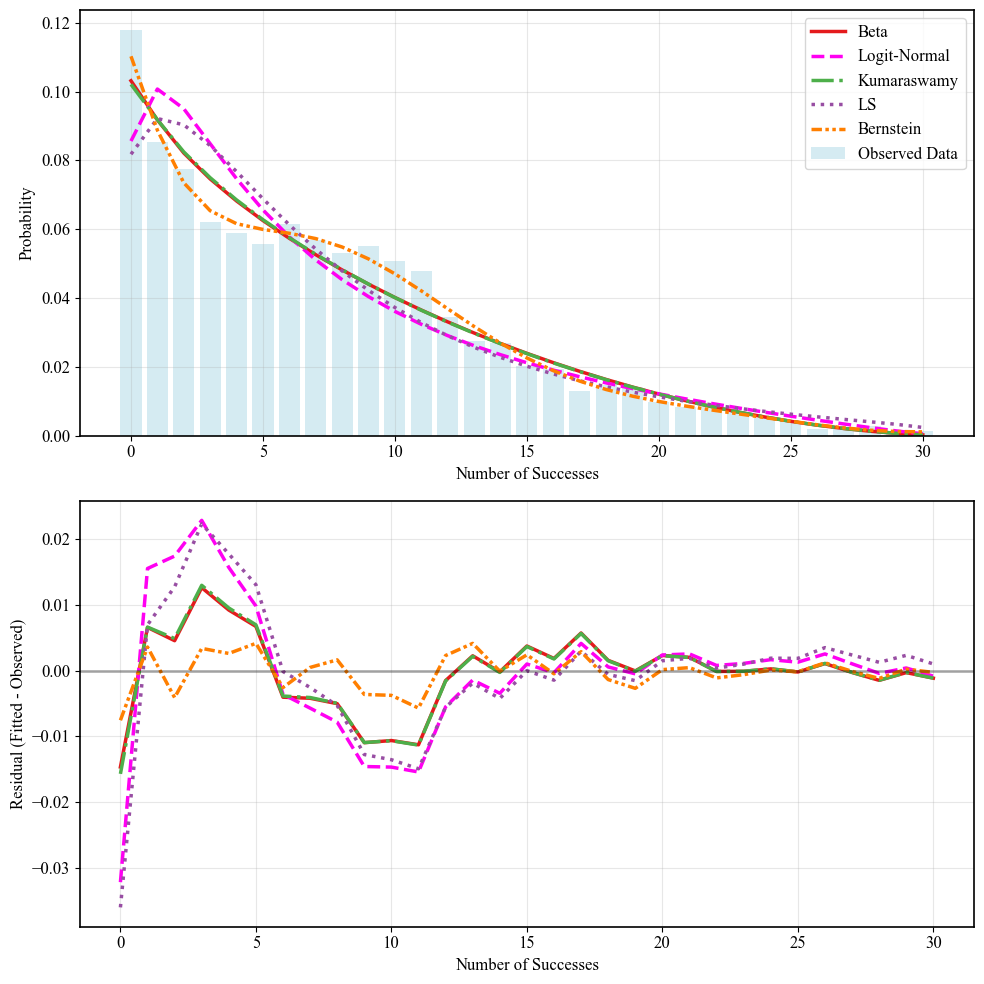
\includegraphics[width=0.479\linewidth]{figures/plot12.png}
    }
    \subfigure[$\;$ Case ($\mbox{B}_3$)]
    {
        \centering
        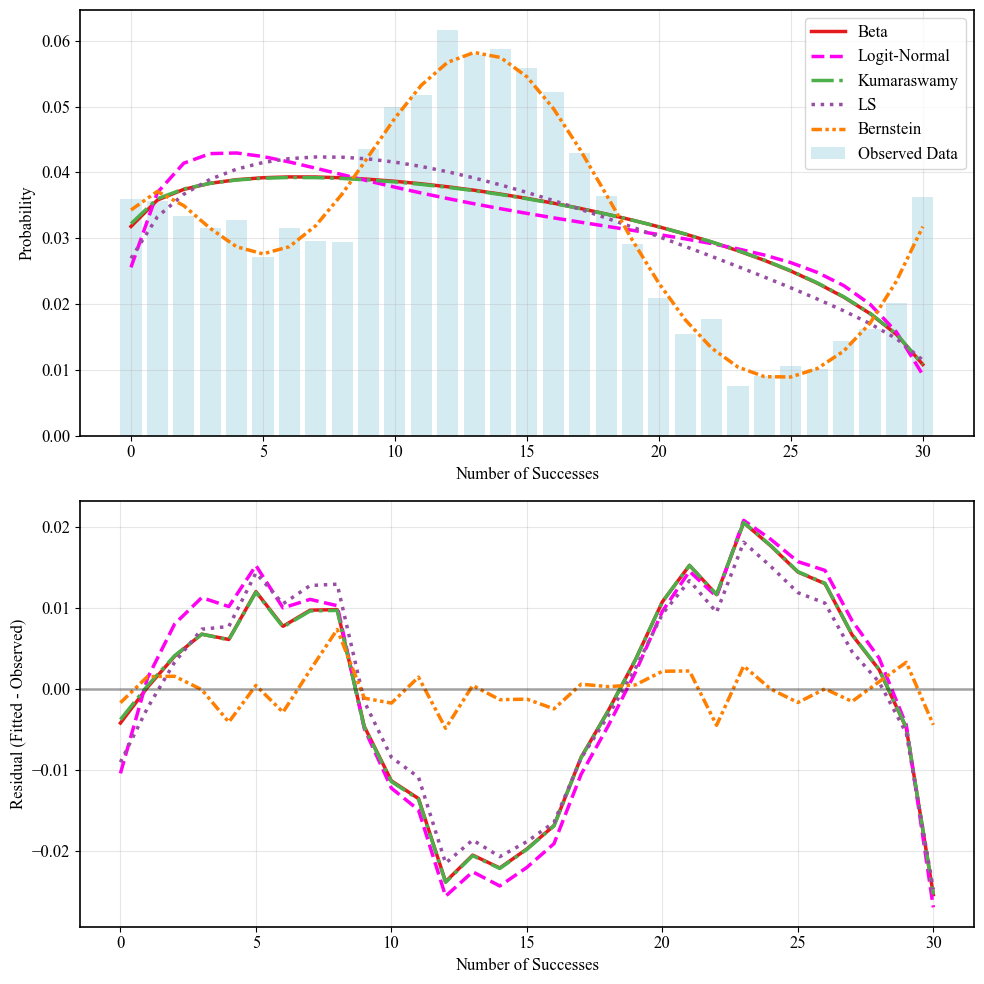
\includegraphics[width=0.479\linewidth]{figures/plot5.png}
    }
    \caption{$\;$ Fitting effect of five distributions and the corresponding residual plots.}
\end{figure}
Figure 2 shows the histogram of the generated samples together with the fitting curve of each distribution, and the residuals of the model fitting, which visually shows the proximity of each model to the empirical distribution. Sub-figure (a) and (b) in Figure 3 uses the Log-likelihood value, AIC, BIC, $p$-value of $\chi^2$ goodness test, \textit{Mean absolute error} (MAE) as evaluation criteria to evaluate the fitting effect of five models, and the comprehensive performance of each distribution are clearly displayed by radar chart. We can see that Bern-Bino has the largest area in the radar chart, which performs best. Sub-figure (c) and (d) represents the Bern-Bino distribution gradually approximates the real distribution with the increase of $K$, showing the flexibility and convergence.
\begin{figure}[H]
    \centering
    \subfigure[$\;$ Radar chart of Case ($\mbox{B}_1$)]
    {
        \centering
        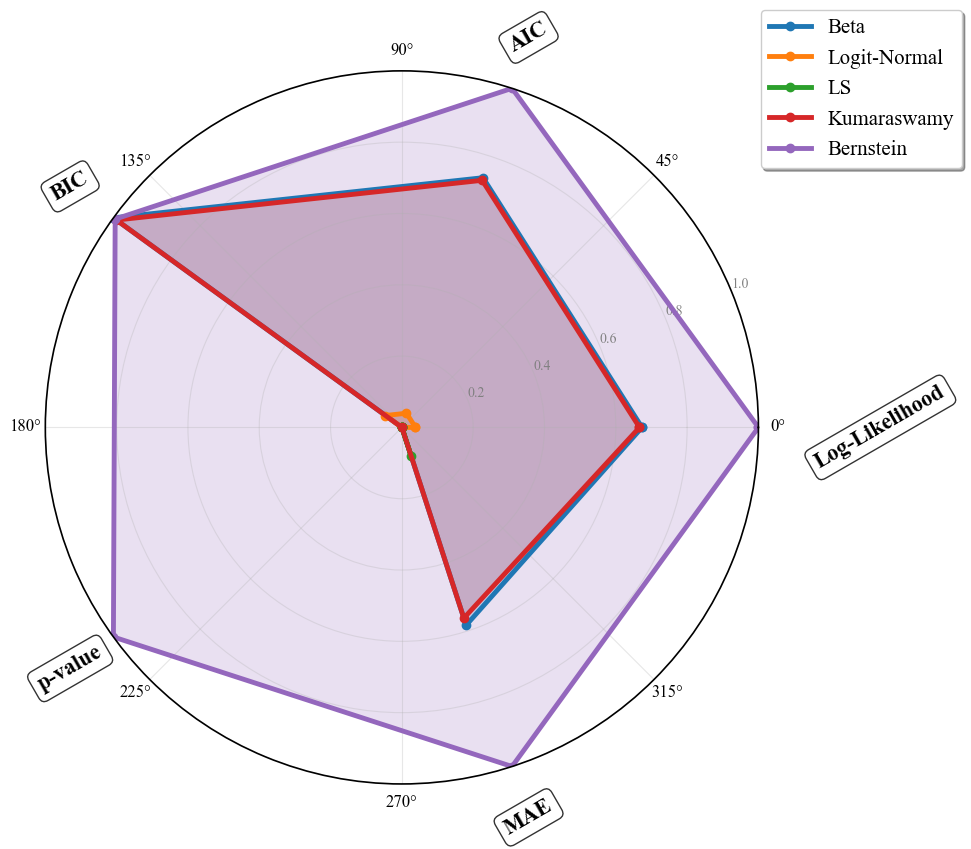
\includegraphics[width=0.479\linewidth]{figures/plot13.png}
    }
    \subfigure[$\;$ Radar chart of Case ($\mbox{B}_3$)]
    {
        \centering
        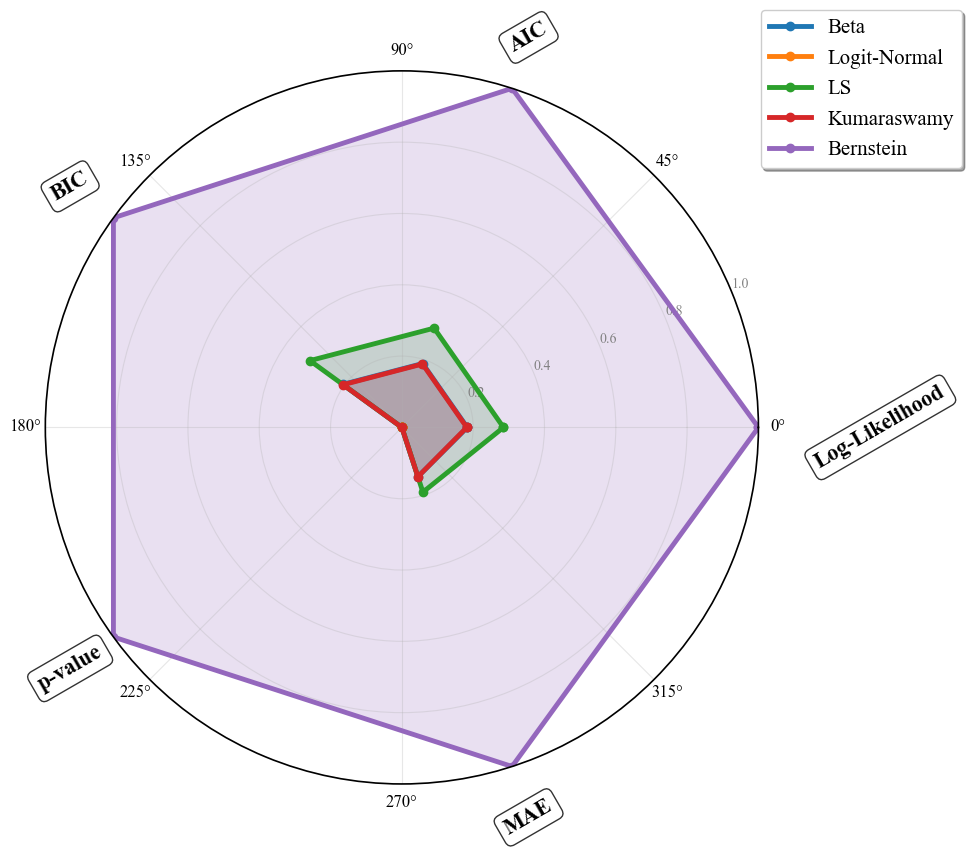
\includegraphics[width=0.479\linewidth]{figures/plot6.png}
    }
    \subfigure[$\;$ Bernstein approximation of Case ($\mbox{B}_1$)]
    {
        \centering
        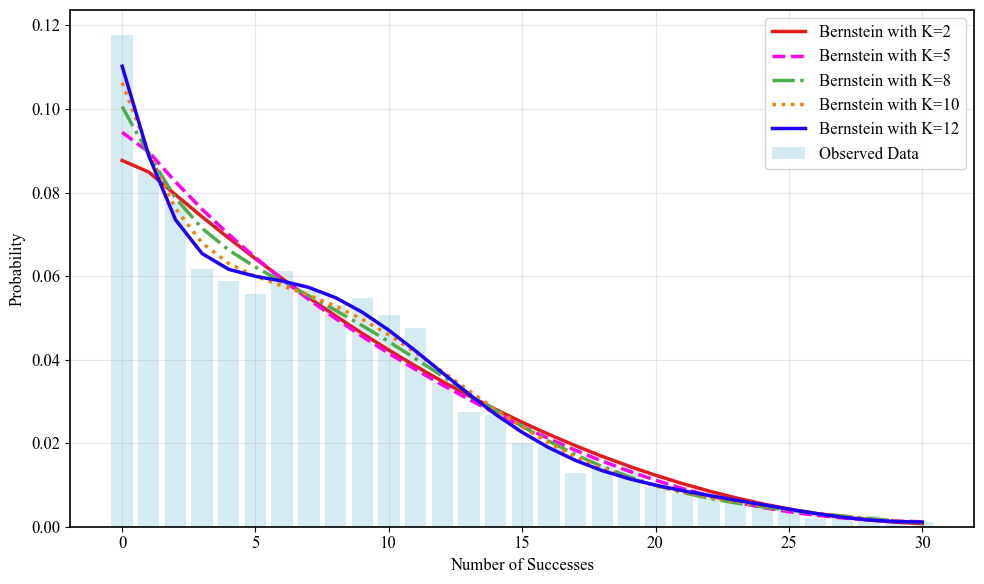
\includegraphics[width=0.479\linewidth]{figures/plot14.png}
    }
    \subfigure[$\;$ Bernstein approximation of Case ($\mbox{B}_3$)]
    {
        \centering
        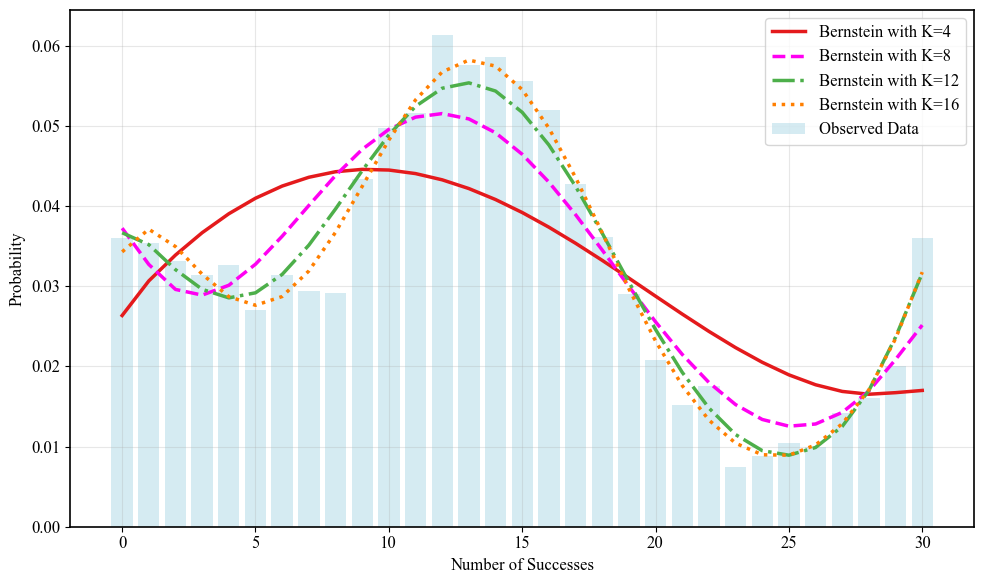
\includegraphics[width=0.479\linewidth]{figures/plot15.png}
    }
    \caption{$\;$ Model comparison for five distributions and Bernstein approximation plots.}
\end{figure}

\subsection{Bayesian inference with DA algorithm}       % Section 3.3

This section will systematically evaluate the performance of Bayesian inference based on DA algorithm in Bern--Bino distribution through numerical simulation. We will evaluate the performance of the posterior mean $\bar{\bla}$ as a point estimator, the coverage and accuracy of Bayesian credible interval (BCI), the convergence and sampling efficiency of DA algorithm and analyze the impact of different Dirichlet prior settings on the posterior inference.

We will construct multiple simulation scenarios to comprehensively evaluate the performance of the algorithm by controlling the sample size $n$ (Factor 1), the real distribution shape $\bla$ (Factor 2) and the Dirichlet prior parameter $\bal$ (Factor 3). For each scenario determined by Factor 1, 2 and 3, we will implement DA algorithm with the number of replications $R=$ 1,000 and collect evaluation indicators for statistical analysis.

Determine the Bernoulli trial number $m=15$ in binomial distribution, the following two different real parameter vectors will be considered:
\begin{namelist}{012345678901234}
\item[\hspace*{-0.05cm} Scenario 1 ($\mbox{S}_1$):] Symmetrical case with $\bla_\text{true} = (0.3, 0.4, 0.3)^{\T}$;

\item[\hspace*{-0.05cm} Scenario 2 ($\mbox{S}_2$):] Skewness with $\bla_\text{true} = (0.25, 0.45, 0.3)^{\T}$.
\end{namelist}
For each scenario, we generate datasets with various sample sizes of $n=200,500,800$ and perform Bayesian inference by using three different Dirichlet priors:
\begin{namelist}{0123456789012}
\item[\hspace*{-0.05cm} Prior 1 ($\mbox{P}_1$):] Non-informative prior with $\bal = \1$;

\item[\hspace*{-0.05cm} Prior 2 ($\mbox{P}_2$):] Correct prior with $\bal = 5 \times \bla_\text{true}$;

\item[\hspace*{-0.05cm} Prior 3 ($\mbox{P}_3$):] Error prior with $\bal = (5, 1, 5)^{\T}$.
\end{namelist}

For each experimental setup determined by $\{\mbox{S}, n, \mbox{P}, r\}$ in $r = 1, \ldots, R$, we run $M = 4$ independent Markov chains. Starting from different random initial values, each chain performs $G = $ 10,000 iterations, discards the previous $B = $ 2,500 as the burn-in period, and retains the last 7,500 samples for analysis. After the iteration, we combine the four chains to get a posterior sample with a size of 30,000. Based on the combined posterior samples, the posterior mean $\bar{\bla}$, bias, 95\% Bayesian credible interval (BCI), interval width, effective sample size (ESS) and Gelman--Rubin convergent diagnostic statistics (R-hat) can be calculated. By independently repeating $R$ experiments, we can calculate the average of each index, the MSE of the posterior mean and the coverage rate \textsf{CR} of BCI.

\begin{figure}[H]
    \centering
    \subfigure[$\;$ Absolute bias and MSE]
    {
        \centering
        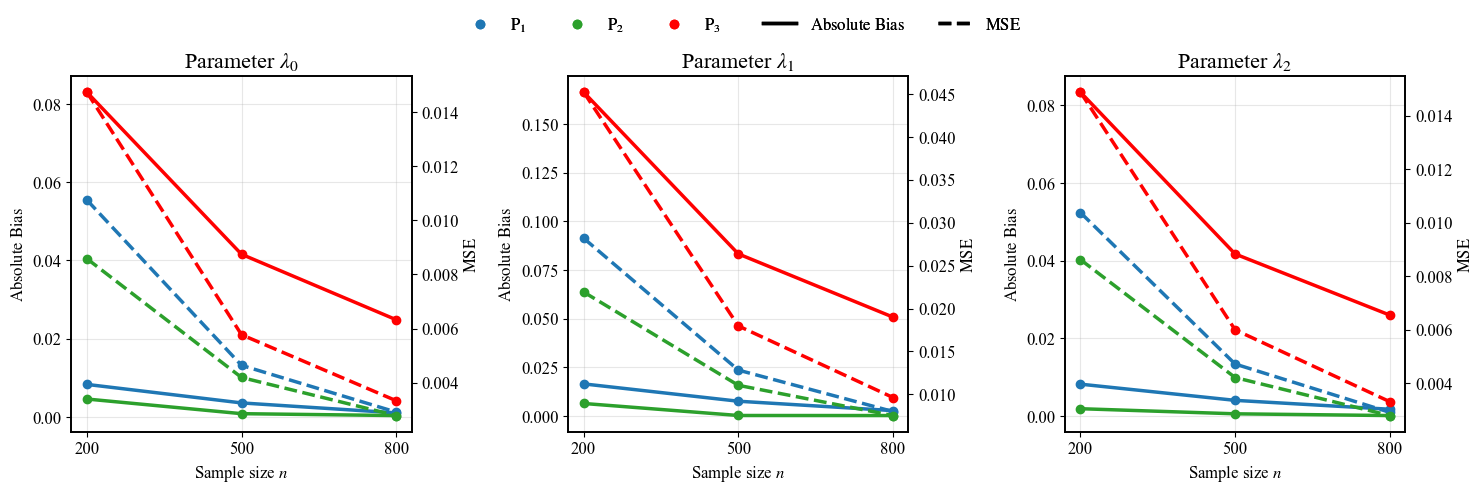
\includegraphics[width=1\linewidth]{figures/plot8.png}
    }
    \subfigure[$\;$ Coverage rate and interval width]
    {
        \centering
        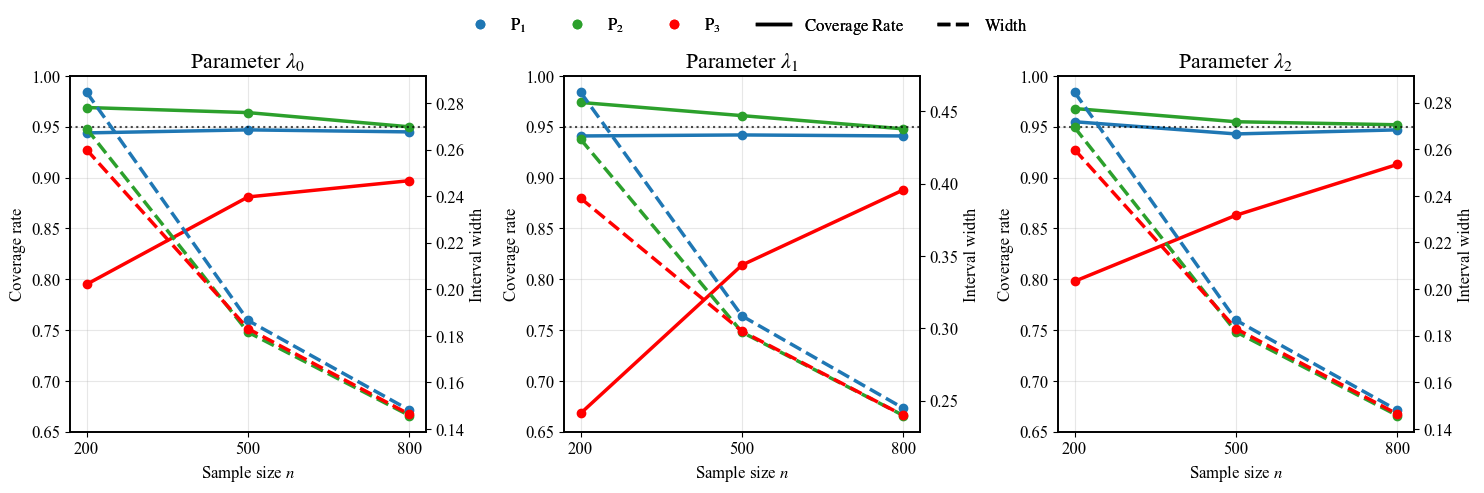
\includegraphics[width=1\linewidth]{figures/plot9.png}
    }
    \caption{$\;$ Performance indicators versus sample size under different priors for $\mbox{S}_1$.}
\end{figure}

Figure 4 shows us the absolute bias and MSE of the posterior mean $\bar{\bla}$, the coverage rate and interval width of 95\% BCIs with the sample size $n$ under different priors in Scenario 1. From the figure, we can found that the absolute bias and MSE decrease with the increase of sample size, and the correct prior information can improve the estimation accuracy especially in the case of small samples. For BCI, the interval width will decrease with the increase of the sample size, and the coverage rate of the correct prior ($\mbox{P}_2$) is the closest to the ideal value, while the coverage rate of the wrong prior ($\mbox{P}_3$) is obviously low when the $n$ is small, and the impact will weaken with the increase of $n$. Figure 5 presents the average coverage rate of $\bla$ for each prior under various sample sizes by employing the radar chart, where we can intuitively observe the above conclusions.

\begin{figure}[H]
    \centering
    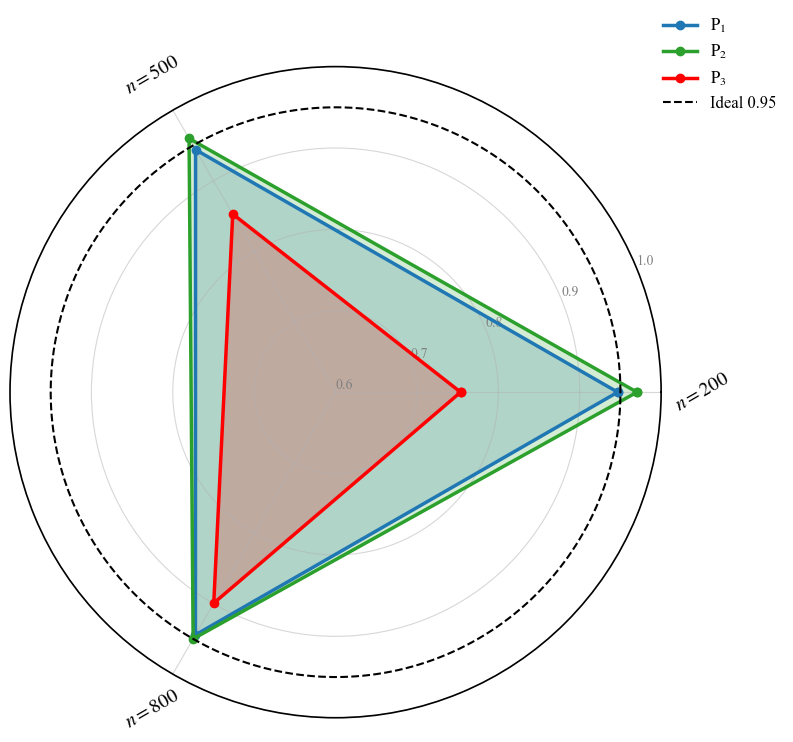
\includegraphics[width=0.65\linewidth]{figures/plot10.png}
    \caption{Radar chart of Coverage rate performance for $\mbox{S}_1$.}
\end{figure}

ESS is an indicator to measure the sampling efficiency of MCMC, which converts the MCMC sample chain with autocorrelation into an equivalent independent sample size, which is calculated based on the sum of the sample autocorrelation function (ACF):
$$
    \mbox{ESS} = \frac{N}{1 + 2 \sum_{t=1}^\infty \rho_t},
$$
where $N$ is the total number of MCMC samples and $\rho_t$ is the autocorrelation coefficient of samples with an interval of $t$. In practice, the sum is usually truncated when $\rho_t$ becomes insignificant. And the Gelman--Rubin statistic $\hat{R}$ (Gelman \& Rubin, 1992) is used to diagnose the convergence of MCMC sampling. The statistic is constructed by comparing the inter chain variance ($B$) and intra chain variance ($W$) of multiple parallel Markov chains. We calculate the corrected total variance estimate
$$
    \widehat{\Var}(\bla) = \frac{N-1}{N} W + \frac{1}{N} B,
$$
then the Gelman--Rubin statistic is $\hat{R} = \sqrt{\widehat{\Var}(\bla)/W}$. When the $\hat{R}$ drops below 1.05 even 1.01, it is generally considered that convergence is sufficient.

\begin{figure}[H]
    \centering
    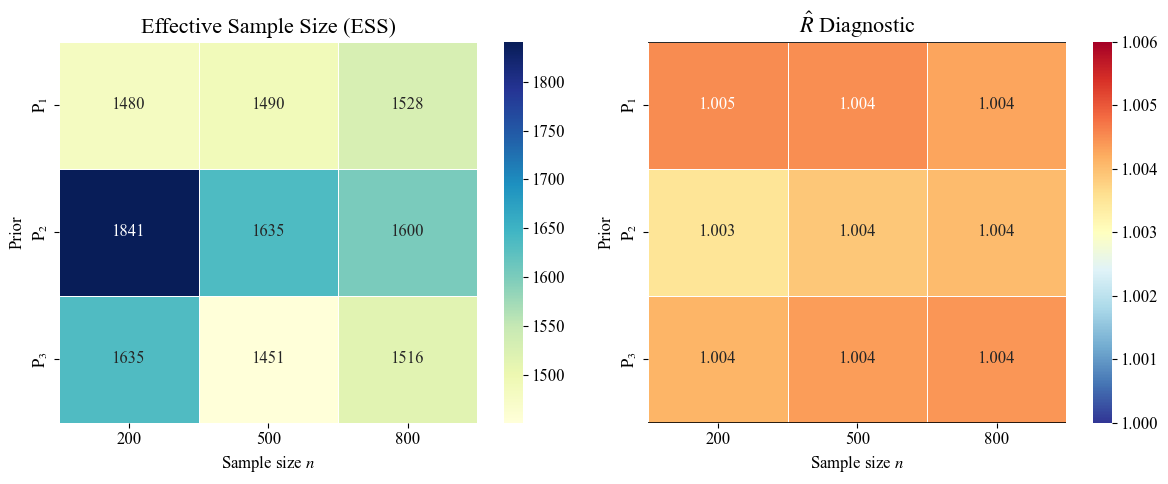
\includegraphics[width=1\linewidth]{figures/plot11.png}
    \caption{Heat map of DA algorithm efficiency for $\mbox{S}_1$.}
\end{figure}

Figure 6 exhibits the ESS and $\hat{R}$ values of DA algorithm under different sample sizes and priors by adopting heatmap. We can find that the ESS value is greater than $1,$$000$ and $\hat{R}$ is less than 1.01 for each case, which means that the efficiency and reliable convergence of posterior sampling and indicates DA algorithm will not be affected by initial value of sampling. In addition, ESS is significantly larger under the correct the prior and has higher sampling efficiency than other priors. For the scenario 2, we summarize the specific results of Bayesian inference in Table (\ref{tab3}), which demonstrates similar conclusions with scenario 1.

\newpage
\vkU
\baselineskip 0.10in
\begin{Table} \label{tab3} {\rm \hspace{-0.2cm}{\bf .}
Influence of different priors on Bayesian inference for $\mbox{S}_2$ based on $R = $ 1,000 replications under various sample sizes
\vspace{-0.15cm}
\begin{center}
\renewcommand{\arraystretch}{1.2} \tabcolsep 0.11in \doublerulesep 0.2pt
\begin{tabular}{|c|c|c|r|c|c|c|c|c|}  \hline\hline
    Sample size    & Parameter          & Prior        & \MC{1}{c|}{\textsf{Bias}} & \textsf{MSE}    & \textsf{CR} & \textsf{I-Width} & \textsf{ESS}  & $\hat{R}$ \\ \hline
    \MR{9}{*}{200} & \MR{3}{*}{$\la_0$} & $\mbox{P}_1$ &    0.0059                 & 0.0099          & 0.954       & 0.277            & 1685          & 1.00      \\
    \MR{9}{*}{}    & \MR{3}{*}{}        & $\mbox{P}_2$ & $-$0.0014                 & 0.0084          & 0.958       & 0.261            & 2089          & 1.00      \\
    \MR{9}{*}{}    & \MR{3}{*}{}        & $\mbox{P}_3$ &    0.0945                 & 0.0166          & 0.739       & 0.258            & 1887          & 1.00      \\ \cline{2-9}
    \MR{9}{*}{}    & \MR{3}{*}{$\la_1$} & $\mbox{P}_1$ & $-$0.0136                 & 0.0279          & 0.959       & 0.465            & 1172          & 1.01      \\
    \MR{9}{*}{}    & \MR{3}{*}{}        & $\mbox{P}_2$ &    0.0050                 & 0.0229          & 0.957       & 0.428            & 1431          & 1.00      \\
    \MR{9}{*}{}    & \MR{3}{*}{}        & $\mbox{P}_3$ & $-$0.1890                 & 0.0538          & 0.589       & 0.404            & 1144          & 1.01      \\ \cline{2-9}
    \MR{9}{*}{}    & \MR{3}{*}{$\la_2$} & $\mbox{P}_1$ &    0.0076                 & 0.0108          & 0.955       & 0.290            & 1738          & 1.00      \\
    \MR{9}{*}{}    & \MR{3}{*}{}        & $\mbox{P}_2$ & $-$0.0036                 & 0.0094          & 0.953       & 0.271            & 2172          & 1.00      \\
    \MR{9}{*}{}    & \MR{3}{*}{}        & $\mbox{P}_3$ &    0.0946                 & 0.0174          & 0.761       & 0.269            & 1843          & 1.00      \\ \hline
    \MR{9}{*}{500} & \MR{3}{*}{$\la_0$} & $\mbox{P}_1$ &    0.0034                 & 0.0042          & 0.958       & 0.180            & 1733          & 1.00      \\
    \MR{9}{*}{}    & \MR{3}{*}{}        & $\mbox{P}_2$ & $-$0.0010                 & 0.0038          & 0.964       & 0.176            & 1885          & 1.00      \\
    \MR{9}{*}{}    & \MR{3}{*}{}        & $\mbox{P}_3$ &    0.0423                 & 0.0057          & 0.865       & 0.177            & 1788          & 1.00      \\ \cline{2-9}
    \MR{9}{*}{}    & \MR{3}{*}{$\la_1$} & $\mbox{P}_1$ & $-$0.0063                 & 0.0124          & 0.954       & 0.305            & 1208          & 1.00      \\
    \MR{9}{*}{}    & \MR{3}{*}{}        & $\mbox{P}_2$ &    0.0025                 & 0.0105          & 0.967       & 0.295            & 1306          & 1.00      \\
    \MR{9}{*}{}    & \MR{3}{*}{}        & $\mbox{P}_3$ & $-$0.0851                 & 0.0177          & 0.812       & 0.295            & 1200          & 1.01      \\ \cline{2-9}
    \MR{9}{*}{}    & \MR{3}{*}{$\la_2$} & $\mbox{P}_1$ &    0.0029                 & 0.0048          & 0.950       & 0.188            & 1783          & 1.00      \\
    \MR{9}{*}{}    & \MR{3}{*}{}        & $\mbox{P}_2$ & $-$0.0015                 & 0.0043          & 0.956       & 0.183            & 1946          & 1.00      \\
    \MR{9}{*}{}    & \MR{3}{*}{}        & $\mbox{P}_3$ &    0.0427                 & 0.0061          & 0.867       & 0.185            & 1796          & 1.00      \\ \hline
    \MR{9}{*}{800} & \MR{3}{*}{$\la_0$} & $\mbox{P}_1$ &    0.0017                 & 0.0027          & 0.944       & 0.143            & 1767          & 1.00      \\
    \MR{9}{*}{}    & \MR{3}{*}{}        & $\mbox{P}_2$ & $-$0.0016                 & 0.0026          & 0.952       & 0.141            & 1856          & 1.00      \\
    \MR{9}{*}{}    & \MR{3}{*}{}        & $\mbox{P}_3$ &    0.0303                 & 0.0034          & 0.872       & 0.142            & 1807          & 1.00      \\ \cline{2-9}
    \MR{9}{*}{}    & \MR{3}{*}{$\la_1$} & $\mbox{P}_1$ & $-$0.0028                 & 0.0077          & 0.947       & 0.242            & 1229          & 1.00      \\
    \MR{9}{*}{}    & \MR{3}{*}{}        & $\mbox{P}_2$ &    0.0025                 & 0.0073          & 0.939       & 0.237            & 1287          & 1.00      \\
    \MR{9}{*}{}    & \MR{3}{*}{}        & $\mbox{P}_3$ & $-$0.0586                 & 0.0103          & 0.857       & 0.237            & 1223          & 1.00      \\ \cline{2-9}
    \MR{9}{*}{}    & \MR{3}{*}{$\la_2$} & $\mbox{P}_1$ &    0.0011                 & 0.0029          & 0.946       & 0.149            & 1813          & 1.00      \\
    \MR{9}{*}{}    & \MR{3}{*}{}        & $\mbox{P}_2$ & $-$0.0009                 & 0.0028          & 0.941       & 0.147            & 1912          & 1.00      \\
    \MR{9}{*}{}    & \MR{3}{*}{}        & $\mbox{P}_3$ &    0.0283                 & 0.0035          & 0.900       & 0.147            & 1827          & 1.00      \\ \hline \hline
\end{tabular}
\end{center} }
\end{Table}
\baselineskip 0.30in 